% Общий объем раздела 25-30 стр.

\section{Разработка и реализация алгоритмов стегоанализа изображений с использованием свёрточных искусственных нейронных сетей}

Машина опорных векторов дала мощный толчок появлению всё более совершенных стегоаналитических методов, однако со временем стегоаналитики ощутили несовершенство практики ручного выделения признаков, и для автоматизации данной процедуры стали использоваться свёрточные нейронные сети.

Пространства признаков, построенные нейронными сетями, по многим параметрам превосходят сконструированные вручную. Благодаря автоматизации их извлечения, размерность пространства признаков зависит не от возможностей стегоаналитика, а от вычислительной мощности используемого аппаратного обеспечения. К тому же, многие признаки довольно сложно получить аналитически ввиду неочевидности статистических зависимостей между элементами контейнеров. Свёрточные нейронные сети на примере задач распознавания образов доказывают свою способность к построению таких признаков. Наконец, метод обратного распространения ошибки~\cite{BackProp} реализует обратную связь, позволяющую конструировать признаки непосредственно во время обработки тренирующей выборки с учётом ошибки классификации, что исключает временные затраты на итеративную процедуру формирования пространства признаков целиком, его тестирования и последующего исправления.

\subsection{Описание нейросетевого подхода и общей схемы алгоритма}

Одной из первых работ, положивших начало нейросетевому подходу к решению задач классификации, стал линейный перцептрон Фрэнка Розенблатта~\cite{Rosenblatt1, Rosenblatt2}. По сути своей перцептрон Розенблатта --- это линейная модель бинарной классификации, задача которой --- научиться сопоставлять метки классов не участвовавшим в обучении объектам.

Будем считать, что каждый вход представляет собой вектор вещественных чисел $ \boldsymbol{x} = (x^1, x^2, \ldots, x^n) \in \mathbb{R}^n $, и входы в тренировочном множестве снабжены известными выходами $ y(\boldsymbol{x}) \in \{-1, +1\} $. Тогда для решения задачи необходимо найти такие веса $ w_0, w_1, \ldots, w_n \in \mathbb{R}^n $, чтобы знак линейной функции
\begin{equation}
sign(w_0 + w_1x^1 + w_2x^2 + \ldots + w_nx^n)
\label{eq:OLPOutput}
\end{equation}
как можно чаще совпадал с правильным ответом $ y(\boldsymbol{x}) $. Положительное значение~\ref{eq:OLPOutput} интерпретируют как суждение о принадлежности $ \boldsymbol{x} $ к классу с меткой $ +1 $, и наоборот.

Для удобства увеличим размерность вектора $ \boldsymbol{x} $ таким образом, чтобы он принял вид $ \boldsymbol{x} = (1, x^1, x^2, \ldots, x^n) \in \mathbb{R}^{n + 1} $. Это позволит считать линейную комбинацию $ w_0 + w_1x^1 + w_2x^2 + \ldots + w_nx^n $ скалярным произведением $ \langle \boldsymbol{w}, \boldsymbol{x} \rangle $, где $ \boldsymbol{w} = (w_0, w_1, w_2, \ldots, w_n) $. Архитектура однослойного перцептрона представлена на рисунке~\ref{fig:OneLayerPerceptron}.

\begin{figure}[h]
\centering
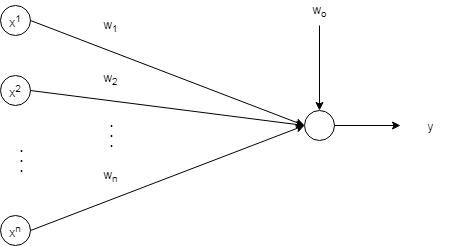
\includegraphics[width=1\textwidth]{include/graphics/one-layer_perceptron}
\caption{Архитектура однослойного перцептрона}
\label{fig:OneLayerPerceptron}
\end{figure}

Для обучения данной функции необходимо выбрать функцию ошибки. Розенблатт вводит в этом качестве \textit{критерий перцептрона}:
\begin{equation}
E_P(\boldsymbol{w}) = - \sum_{\boldsymbol{x} \in \mathcal{M}} y(\boldsymbol{x}) \langle \boldsymbol{w}, \boldsymbol{x} \rangle,
\label{eq:PerceptronCriterion}
\end{equation}
где $ \mathcal{M} $ обозначает множество множество примеров, которые перцептрон с весами $ \mathbf{w} $ классифицирует неверно.

Оптимизировать~\ref{eq:PerceptronCriterion} можно методом градиентного спуска, согласно которому вектор весов на шаге обучения~$ \tau $ имеет следующий вид:
\begin{equation*}
\boldsymbol{w}^{(\tau + 1)} = \boldsymbol{w}^{(\tau)} - \eta\nabla_{\boldsymbol{w}}E_P(\boldsymbol{w}).
\end{equation*}

Такой классификатор способен работать только с линейно разделимыми множествами. Популярным антипримером использования перцептрона Розенблатта является т. н. проблема XOR: множество нулей и множество единиц данной функции линейно неразделимы. Ввиду линейности конструкции объединение нескольких таких нейронов в сеть не имеет смысла: композиция линейных функций снова будет линейной, и сеть из любого, сколь угодно большого числа линейных перцептронов сможет реализовать только те же самые линейные функции, для которых было достаточно и одного. Для построения нелинейного классификатора вводят нелинейную функцию активации, принимающую на вход линейную комбинацию $ \boldsymbol{w}, \boldsymbol{x} \rangle $. Наиболее популярная исторически функция активации~--- \textit{логистический сигмоид}:
\begin{equation*}
f(x) = \frac{1}{1 + e^{-x}}.
\end{equation*}

Как и другие функции активации нейронов, это монотонно неубывающая функция, которая при $ x \to -\infty $ стремится к нулю, а при $ x \to +\infty $~--- к единице. Это значит, что при подаче на вход большого по модулю отрицательного числа нейрон не активируется, но активируется при подаче такого же положительного. Более того, данная функция активации равна 0,5 при $ x = 0 $, что вкупе с использованием \textit{перекрёстной энтропии} в качестве функции ошибок позволяет получать на выходе не два дискретных значения -1 и +1, а десятичную дробь в диапазоне $ (0,5; 1) $, означающую вероятность принадлежности $ \boldsymbol{x} $ к классу, ассоциированному с конкретным выходом. Средняя перекрёстная энтропия по всем объектам тренирующей выборки имеет вид:
\begin{equation*}
E_P(\boldsymbol{w}) = -\frac{1}{n} \sum_{i = 1}^n [y(\boldsymbol{x}_i)\ln(f(\langle \boldsymbol{w}, \boldsymbol{x}_i \rangle)) + (1 - y(\boldsymbol{x}_i))\ln(1 - f(\langle \boldsymbol{w}, \boldsymbol{x}_i \rangle))].
\end{equation*}

Перейдём от однослойного перцептрона к многослойной полносвязной нейронной сети. Обозначим выход $ j $\=/того нейрона $ l $\=/того слоя как $ y_j^l $:
\begin{equation*}
y^{j(l)} = f(\sum_{i = 0}^{m_0} w_{ji}^ly^{i(l - 1)}),
\end{equation*}
где $ m_0 $~--- размерность $ l $\=/того слоя, $ w_{ji}^l $~--- вес синаптической связи, соединяющей $ j $\=/тый нейрон слоя $ l $ с $ i $\=/тым нейроном слоя $ l - 1 $.

$ y^{j(0)} = x^j $, где $ x^j $ --- $ j $\=/тый элемент входного вектора.

В данном случае для минимизации значения функции ошибок необходимо подобрать параметры уже не одного нейрона, а всей сети. Для этого используется метод обратного распространения ошибки, являющийся модификацией метода градиентного спуска. В качестве функции ошибок преимущественно используется категориальная перекрёстная энтропия.

\subsubsection{Обзор архитектуры свёрточной нейронной сети}

Свёрточная нейронная сеть обычно состоит из двух блоков: блока свёрточных слоёв и блока полносвязных слоёв, аналогичных слоям многослойного перцептрона. Типовая архитектура свёрточной нейронной сети приведена на рисунке~\ref{fig:CNNArchitectureExample}.

\begin{figure}[h]
\centering
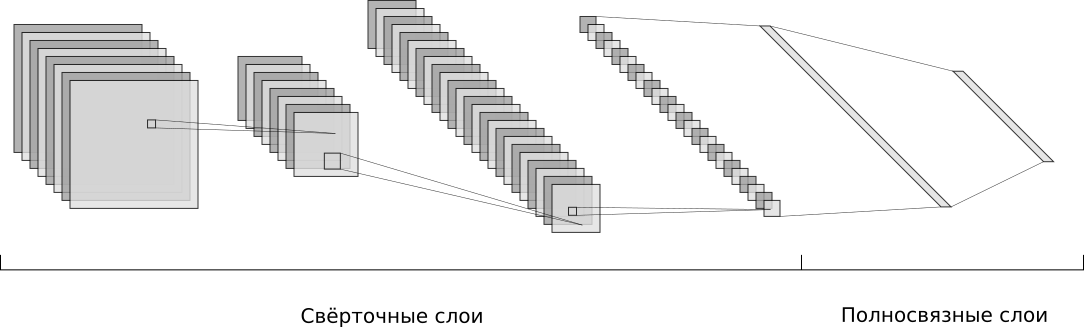
\includegraphics[width=1\textwidth]{include/graphics/cnn_architecture_example}
\caption{Типовая архитектура свёрточной нейронной сети}
\label{fig:CNNArchitectureExample}
\end{figure}

Основная идея свёрточных слоёв заключается в извлечении карт признаков из двумерных матриц с последующей их передачей в классификатор, в роли которого выступает блок полносвязных слоёв. Карты признаков выгоднее для классификации, чем исходные данные, поскольку они имеют меньшую размерность, а их содержанием являются наиболее существенные признаки начальных данных. Это объясняет успех свёрточных нейронных сетей в области распознавания образов и классификации изображений.

Каждый свёрточный слой обычно выполняет три операции для получения карт признаков. Первый шаг --- фильтрация методом скользящего окна с использованием $ K $ ядер, результатом которой является $ K $ карт признаков. Каждое ядро применяется к существующей карте признаков, полученной в предыдущем слое. В первом свёрточном слое все ядра применяются к исходному изображению. Затем производится уменьшение размерности карт признаков с помощью операции субдискретизации (пулинга) путём вычисления среднего или максимального значения в каждом регионе карты признаков размера $ p \times p $. Финальный шаг --- расчёт нелинейной функции карты признаков.

В сравнении с полносвязными слоями свёрточные слои обучаются быстрее ввиду использования метода скользящего окна. Благодаря этому, в обучении нуждаются не все связи между соседними слоями, а только элементы свёрточного ядра, общего для одной конкретной матрицы. Это разделение весов не только существенно уменьшает их количество, но и повышает обобщающие способности сети, позволяя формировать универсальные относительно различных участков изображений свёрточные ядра.

Как и в нейронных сетях других типов, процесс обучения заключается в минимизации функции потерь с использованием оптимизационного алгоритма, обновляющего веса. Пакетный режим стохастического градиентного спуска в качестве оптимизационного алгоритма очень популярен, но AdaDelta или AdaGrad также могут применятся в свёрточных нейронных сетях. 

Рассмотрим детальнее некоторые операции, применяемые в свёрточных слоях.

\textbf{Свёртка.} Обозначим результат свёртки в слое $ l $ с $ k $\=/ым ядром, равным матрице весов $ W^{kl} $, как $ C^{kl} $. Тогда
\begin{equation*}
C^{kl} = \sum_{m = 1}^{K^{l - 1}} (W^{kl} * F^{m(l - 1)}),
\end{equation*}
где $ * $ обозначает операцию свёртки. $ K^{l - 1} $~--- это количество ядер в предыдущем слое, а $ F^{m(l - 1)} $~--- $ k $\=/ая карта признаков, полученная из предыдущего слоя. Для первого свёрточного слоя $ l = 1 $, $ K^{l - 1} = K^0 = 1 $, а $ F^{1(l - 1)} = F^{10} = I $, где $ I $~--- входное изображение. Размер матрицы фильтрации $ W^{kl} $ напрямую определяет размер локальной области (скользящего окна), используемой для вычисления $ C^{kl}_{ij} $.

Размер выходной матрицы также зависит от двух параметров, называемых шагом свёртки и дополнением (англ.~padding). Шаг свёртки $ S $ задаёт дискрет перемещения скользящего окна, регулирующий степень пересечения локальных областей. Дополнение позволяет дополнить входную карту признаков $ F^{m(l - 1)} $ или изображение $ I $ нулями по краям. Обозначим толщину дополнения $ P $.

\begin{equation*}
dim(C^{kl}) = (dim(F^{m(l - 1)}) - dim(W^{kl}) + 2 \times P) / S + 1.
\end{equation*}

Например, для сохранения размерности $ C^{kl} $ равной размерности входных данных $ F^{m(l - 1)} $ ($ dim(C^{kl}) = dim(F^{m(l - 1)} $) необходимо соблюсти условие
\begin{equation*}
\begin{cases}
S = 1, \\
P = dim(W^{kl}/2). \\
\end{cases}
\end{equation*}

\textbf{Функция активации.} Для внесения нелинейности каждый результат свёртки $ C^{kl} $ обрабатывается с помощью функции активации $ f^{kl}: \mathbb{R} \to \mathbb{R} $ так же, как это происходит в других типах нейронных сетей. В качестве функции активации в свёрточных нейронных сетях часто используются логистический сигмоид, гиперболический тангенс $ f(x) = tanh(x) $ и ReLU:
\begin{equation*}
f(x) = max(0, x).
\end{equation*}

\textbf{Субдискретизация (пулинг).} Результатом применения данной операции является уменьшение размерности двумерного массива путём его разбиения на фрагменты размером $ p_l \times p_l $ с последующей заменой каждого фрагмента средним или максимальным значением его элементов. Значение шага регулирует пересечение соседних фрагментов, хотя наиболее часто шагу присваивается значение $ p_l $, и пересечения не происходит. Значение $ p_l $ обычно выбирается в диапазоне от 2 до 5, в зависимости от размерности входных данных слоя $ l $.

Субдискретизация выполняет две функции: на уровне одного слоя --- снижение размерности и путём вычисления «типичного» признака фрагмента или взятия наиболее сильно проявляющегося признака; на уровне сети в целом --- агрегирование низкоуровневых признаков в высокоуровневые.

В задачах стегоанализа выбор операции усреднения при осуществлении субдискретизации оправдан слабым характером стеговоздействия, не позволяющим ему достаточно часто принимать максимальное значение на карте признаков.

Запишем выражение для выхода первого свёрточного слоя:
\begin{align*}
F^{k1} &= pooling(f^{k1}(\sum_{m = 1}^{K^0}(W^{k1} * F^{m(l - 1)}) + b^{k1})) = pooling(f^{k1}(W^{k1}*F^{10} + b^{k1})) \\
&= pooling(f^{k1}(W^{k1} * I + b^{k1})).
\end{align*}

\subsection{Свёрточная нейронная сеть GNCNN}

Модель свёрточной нейронной сети для стегоанализа изображений в оттенках серого GNCNN была предложена в~\cite{GNCNN}. Её основные отличительные особенности: применение фильтра предварительной обработки и использование функции Гаусса в качестве функции активации нейронов свёрточных слоёв.
\begin{equation}
\label{eq:GNCNNConvKernel}
%\begin{align*}
K = \frac{1}{12}
\begin{pmatrix*}[r]
    -1 &  2 &    -2 &  2 & -1 \\
     2 & -6 &     8 & -6 &  2 \\
    -2 &  8 & -12 &  8 & -2 \\
     2 & -6 &     8 & -6 &  2 \\
    -1 &  2 &    -2 &  2 & -1 \\
\end{pmatrix*}
%\end{align*}
\end{equation}

Полосовой высокочастотный фильтр предварительной обработки с импульсной характеристикой~\eqref{eq:GNCNNConvKernel} введён исходя из априорного знания о слабом характере стеговоздействия на стегоконтейнер. Целью предварительной фильтрации является усиление яркости стегосигнала и ослабление яркости оригинального изображения. Веса данного фильтра заранее предопределены и не участвуют в процессе обучения нейронной сети.

Ещё одним преобразованием, облегчающим процесс извлечения признаков, является переход от оригинального изображения к шумоподобному остатку $ R = (r_{ij}) $, содержащему только предсказания относительно факта стеганографической модификации каждого пикселя:
\begin{equation*}
r_{ij} = y_{ij} - P(N(Y, i, j)),
\end{equation*}
где $ Y = (y_{ij}) $ – стегоконтейнер, а $ P(N(Y, i, j)) $ – оценка значения пикселя $ y_{ij} $, полученная из окружающих его пикселей $ N(Y, i, j) $~\cite{FridrichNoiseResidual}. Ввиду наличия сложных зависимостей между соседними пикселями, в случае отсутствия модификации оценка зачастую будет близка к действительному значению пикселя $ y_{ij} $, а значение $ r_{ij} $ будет близко к нулю.
\begin{equation}
\label{eq:GaussianFunction}
%\begin{align*}
f(x) = e^{-\frac{x^2}{\sigma^2}}
%\end{align*}
\end{equation}

Функция Гаусса~\eqref{eq:GaussianFunction} с нулевым математическим ожиданием в качестве функции активации (рис.~\ref{fig:GaussianFunction}) призвана обеспечить формирование в свёрточном слое нейронной сети такого ядра $ K $, что $ Y*K = R $. Максимальное значение функции в нуле соответствует нулевой ошибке оценки значения $ y_{ij} $ и, следовательно, предположению об отсутствии модификации пикселя стегоконтейнера. Резкий спад по мере удаления от нуля обращает в близкие к нулю значения любой результат свёртки, превышающий порог, определяемый среднеквадратическим отклонением $ \sigma $, влияющим на ширину кривой.

\begin{figure}
\centering
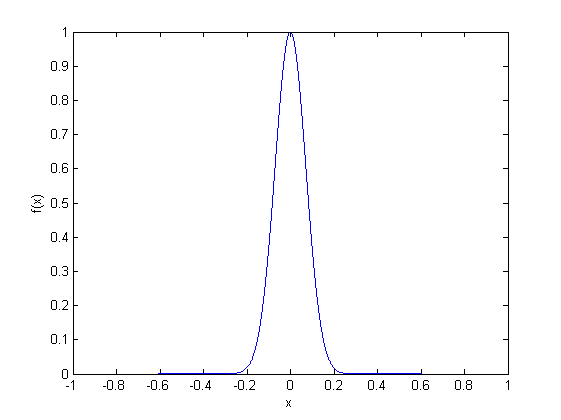
\includegraphics[width=1\textwidth]{include/graphics/gaussian_function}
\caption{Функция активации GNCNN}
\label{fig:GaussianFunction}
\end{figure}

Архитектура нейронной сети представлена на рис.~\ref{fig:GNCNNArchitecture} и имеет вид состояний, через которые проходит входное изображение. Между состояниями располагаются порядковые номера слоёв.

\begin{figure}
\centering
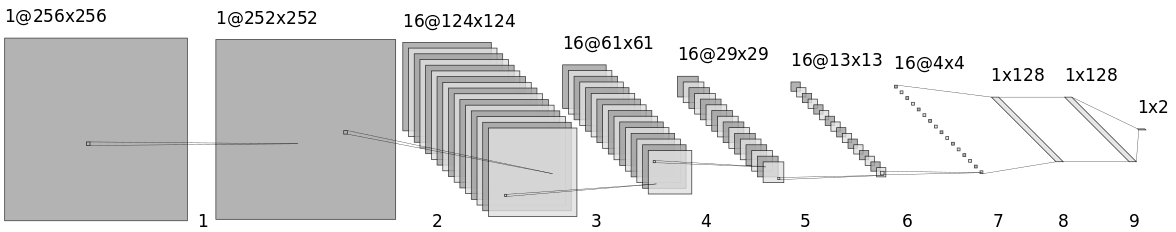
\includegraphics[width=1\textwidth]{include/graphics/gncnn_gray_architecture}
\caption{Архитектура GNCNN}
\label{fig:GNCNNArchitecture}
\end{figure}

На вход нейронной сети подаётся изображение в оттенках серого в разрешении 256×256 пикселей. Слой предварительной обработки 1 с ядром~\eqref{eq:GNCNNConvKernel} не участвует в обучении. За ним следуют пять свёрточных слоёв 2--6, состоящих из 16 каналов. Каждый из них осуществляет операцию свёртки с ядрами, формирующимися по мере обучения сети, а также вычисление функции активации и выполнение субдискретизации по среднему с размером окна 3×3 и шагом 2. Слой 2 использует для свёртки ядра размера $ 5 \times 5 $, слои 3--5 --- ядра размера $ 3 \times 3 $, слой 6 --- ядра размера $ 5 \times 5 $.

Выход последнего свёрточного слоя представляет собой 256 выделенных признака. Они помещаются в модуль классификации, состоящий из трёх полносвязных слоёв 7--9: первые два имеют по 128 нейронов каждый и функцию активации ReLU, последний – два нейрона и функцию активации softmax. В качестве функции потерь используется перекрёстная энтропия.

\subsection{Нейронная сеть с двумя свёрточными слоями}

Также в рамках работы была реализована модель свёрточной нейронной сети для стегоанализа изображений в оттенках серого, предложенная в~\cite{FrenchCNN}. Её особенностями являются отсутствие процедуры субдискретизации и размер свёрточного слоя, располагающегося непосредственно перед полносвязным:
\begin{equation*}
dim(W^{k(L - 1)}) = dim(C^{k(L - 2)}) - 1.
\end{equation*}

Тогда при $ S = 1$ и $ P = 0 $
\begin{equation*}
dim(C^{k(L - 1)}) = (dim(C^{k(L - 2)}) - (dim(C^{k(L - 2)}) - 1) / S + 1 = 2.
\end{equation*}

Таким образом, свёрточный слой $ C^{k(L - 1)} $ выделяет 4 признака на основе зависимостей во всей карте признаков $ dim(F^{k(L - 2)} $, а не отдельных фрагментов, что позволяет детектировать алгоритмы, вносящие слабое искажение, неравномерно распределённое по разным частям контейнера, в отличие от блочных стегоалгоритмов.

Для корректности эксперимента размеры слоёв были изменены для работы со входными изображениями в разрешении 256×256 пикселей. Архитектура нейронной сети приведена на~\ref{fig:FrenchCNNArchitecture}.

% Рисунок 1.4 -- French CNN Architecture
\begin{figure}[!htb]
\centering
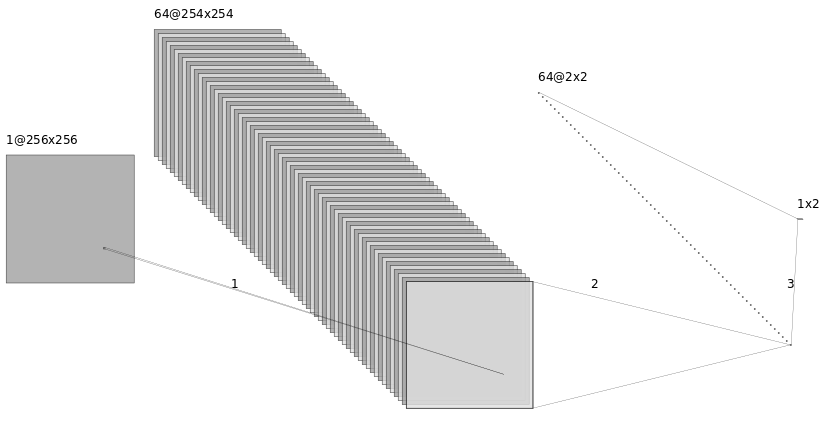
\includegraphics[width=1\textwidth]{include/graphics/french_gray_architecture}
\caption{Архитектура сети с двумя свёрточными слоями}
\label{fig:FrenchCNNArchitecture}
\end{figure}

На вход нейронной сети подаётся изображение в оттенках серого в разрешении 256×256 пикселей. Первый свёрточный слой имеет размер 3×3. Его цель --- произвести высокочастотную фильтрацию подобно тому, как это делает фильтр предварительной обработки GNCNN. Замена константного ядра обучаемым мотивирована отсутствием доказательства оптимальности ядра~\ref{eq:GNCNNConvKernel}. Далее следует свёрточный слой размера 253×253, состоящий из 64 каналов. Оба свёрточных слоя осуществляют операцию свёртки с обучаемым ядром и вычисление функции активации tanh. Результатом их работы являются 64 карты признаков размера 2×2, соединённые с двумя нейронами с функцией активации softmax. В качестве функции потерь используется категориальная кросс-энтропия.

\subsection{Комбинированная свёрточная нейронная сеть}

Рассмотрим архитектуру комбинированной свёрточной сети, совмещающей в себе особенности как GNCNN, так и нейронной сети с двумя свёрточными слоями. Результаты классификации тестовой выборки, приведённые в~\cite{FrenchCNN}, показывают, что большое количество свёрточных слоёв и уменьшение размерности пространства признаков, создаваемого ими, путём применения субдискретизации не являются необходимыми условиями для построения нейросетевого стегоанализатора, хотя увеличивают вычислительную сложность модели нейронной сети.

Сравнение результатов классификации обеих рассмотренных ранее нейронных сетей, а также сравнение эффекта, достигаемого при использовании различных функций активации совместно с архитектурой GNCNN~\cite{Qian2017}, также показали, что функция Гаусса в качестве функции активации свёрточных слоёв не даёт никаких преимуществ в сравнении с традиционно используемыми в свёрточных нейронных сетях функциями активации.

Однако, сильной стороной GNCNN является использование фильтра предварительной обработки, увеличивающего скорость сходимости градиентного обучения.

Учитывая вышеперечисленные выводы, для комбинированной свёрточной сети было решено использовать архитектуру нейронной сети с двумя свёрточными слоями, но с добавлением предварительной фильтрации, описанной в~\cite{GNCNN}. В качестве функции ошибки была выбрана перекрёстная энтропия с $ L_2 $-регуляризацией~\cite{Tikhonov}. Конечная архитектура показана на рисунке~\ref{fig:MixedCNNArchitecture}.

\begin{figure}[!htb]
\centering
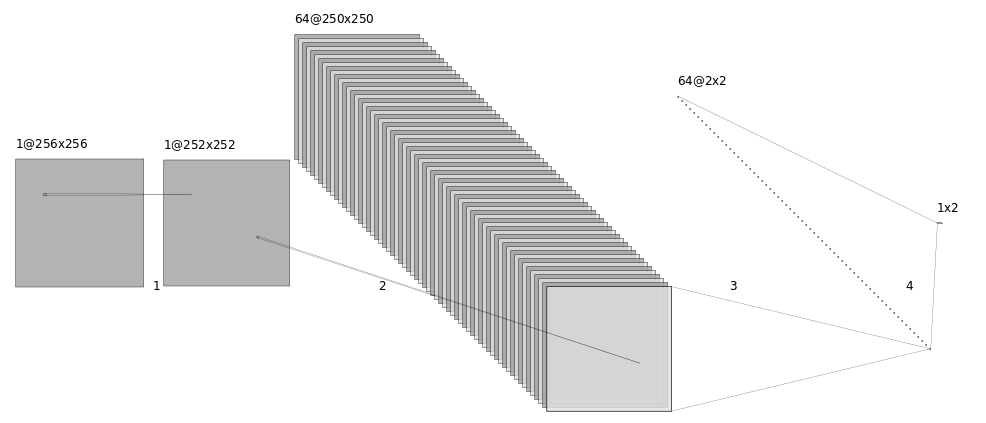
\includegraphics[width=1\textwidth]{include/graphics/mixed_gray_architecture}
\caption{Архитектура комбинированной свёрточной сети}
\label{fig:MixedCNNArchitecture}
\end{figure}

\clearpage
